\section{Dataset 2: Pima Indians Diabetes Dataset (Classification)}

Regarding data processing, several things were done to improve the dataset. Firstly, the target variable was converted from text strings to binary. The \textit{Skin Thickness} and \textit{Insulin} features lacked many rows of measurements; as such, these were discarded. Despite this, some measurements had 0 values that were equivalent to impossible; the rows containing these were discarded. The remaining data processing tasks were already implemented. The performance metrics improved after these measures were implemented.

Fuzzy C-Means Clustering was applied with a range of values for the number of clusters of 2 to 10 with an increment of 1 and the fuzziness coefficient was varied between 1.5 and 2.5 with an increment of 0.1. The results were evaluated using the Fuzzy Partition Coefficient (FPC) and culminated in a number of 2 clusters and a fuzziness coefficient of 1.5 achieving a FPC of 0.7231894414858948.

The resulting TSK model achieved an ACC of 0.8.

\begin{figure}[h!]
    \centering
    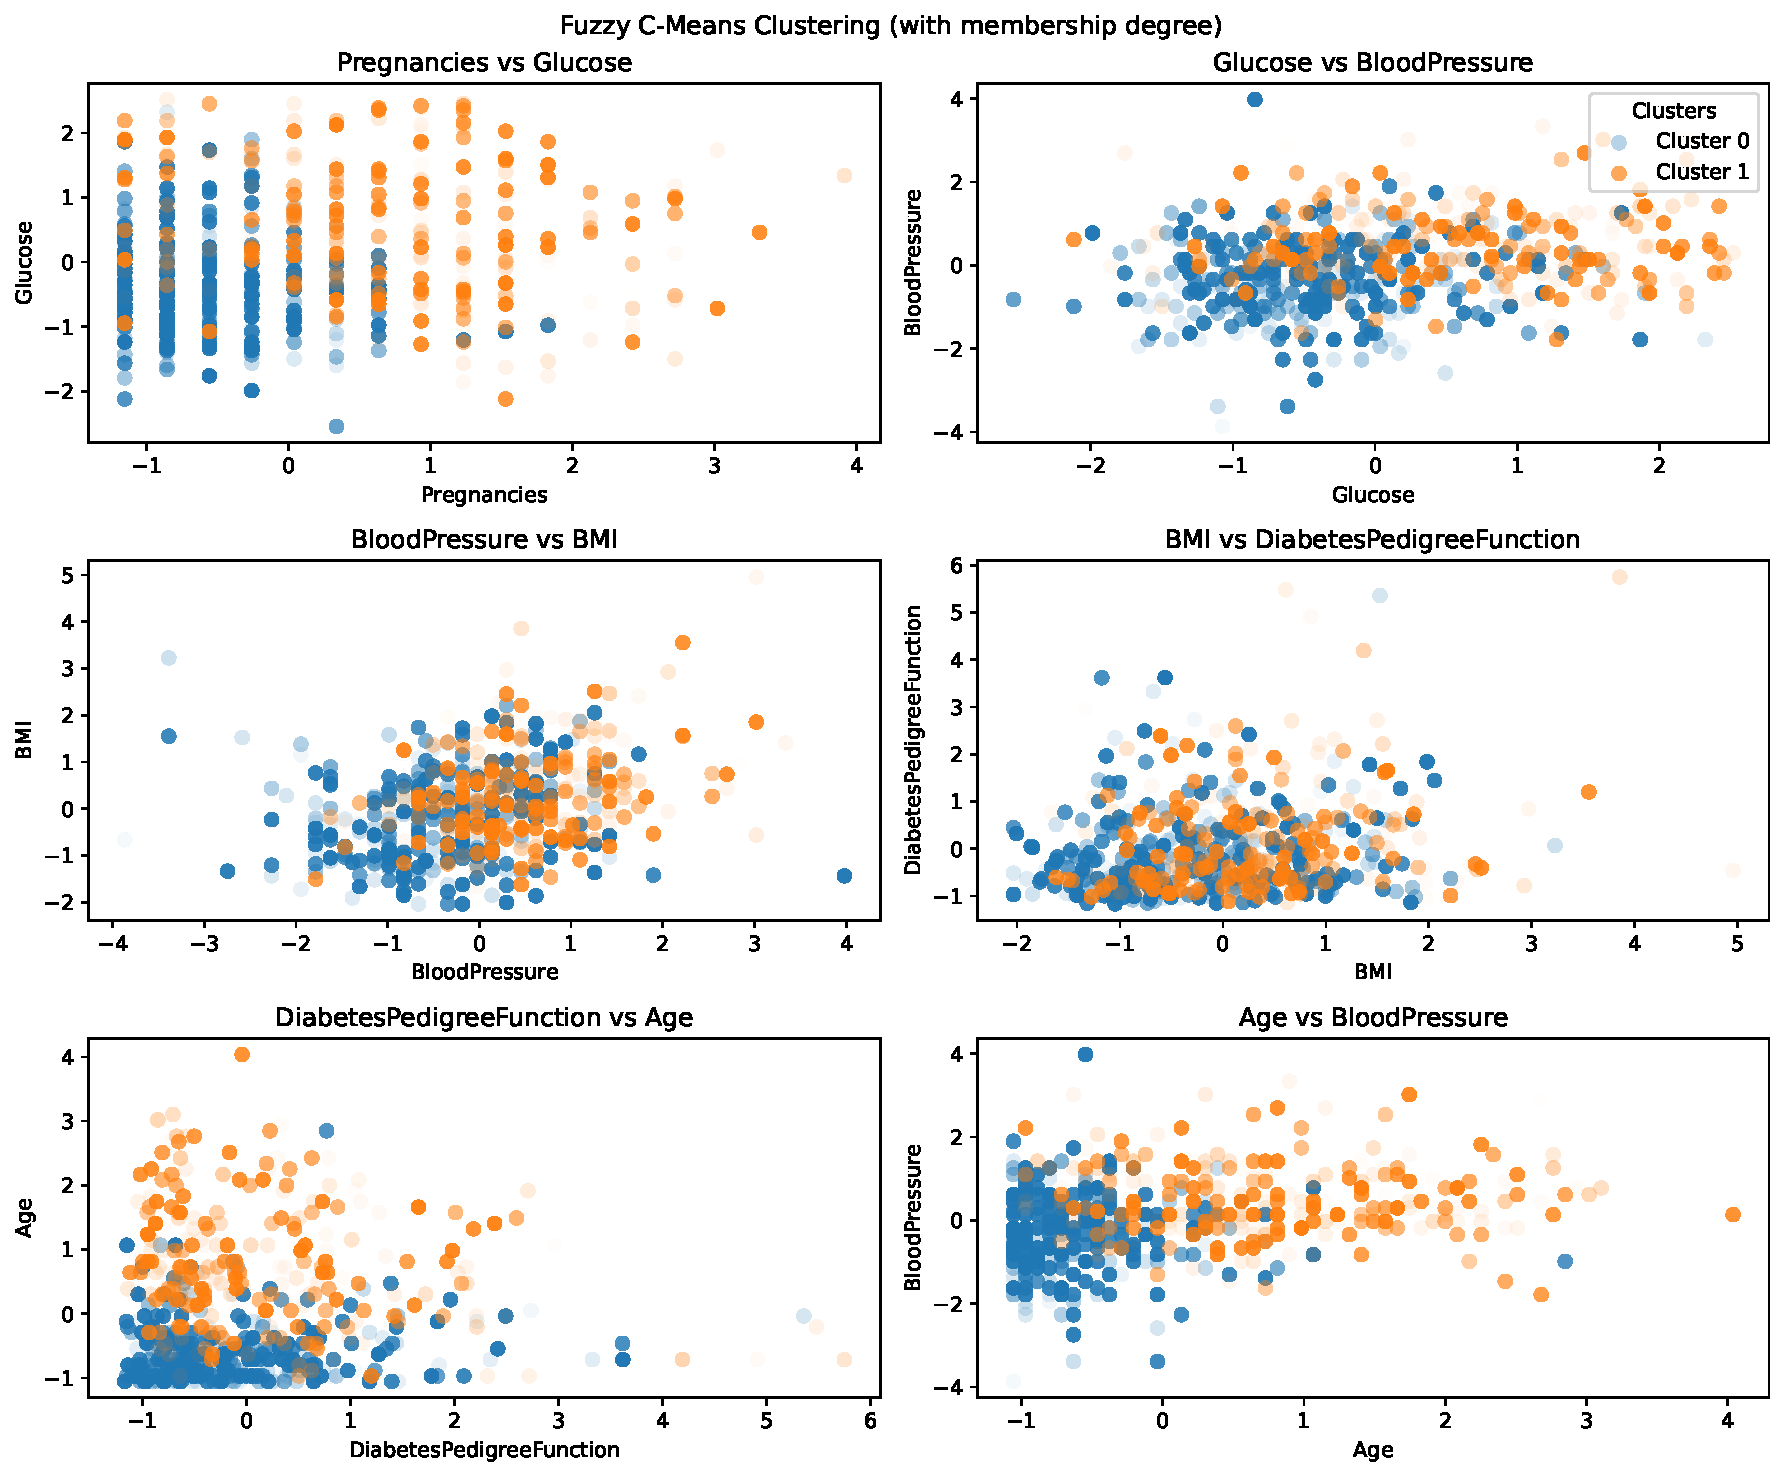
\includegraphics[width=1\textwidth]{Plots/Fuzzy C-Means Clustering (with membership degree) CLF.pdf}
    \caption{Fuzzy C-Means Clustering (with membership degree)}
    \label{fig:my_label}
\end{figure}

\begin{figure}[h!]
    \centering
    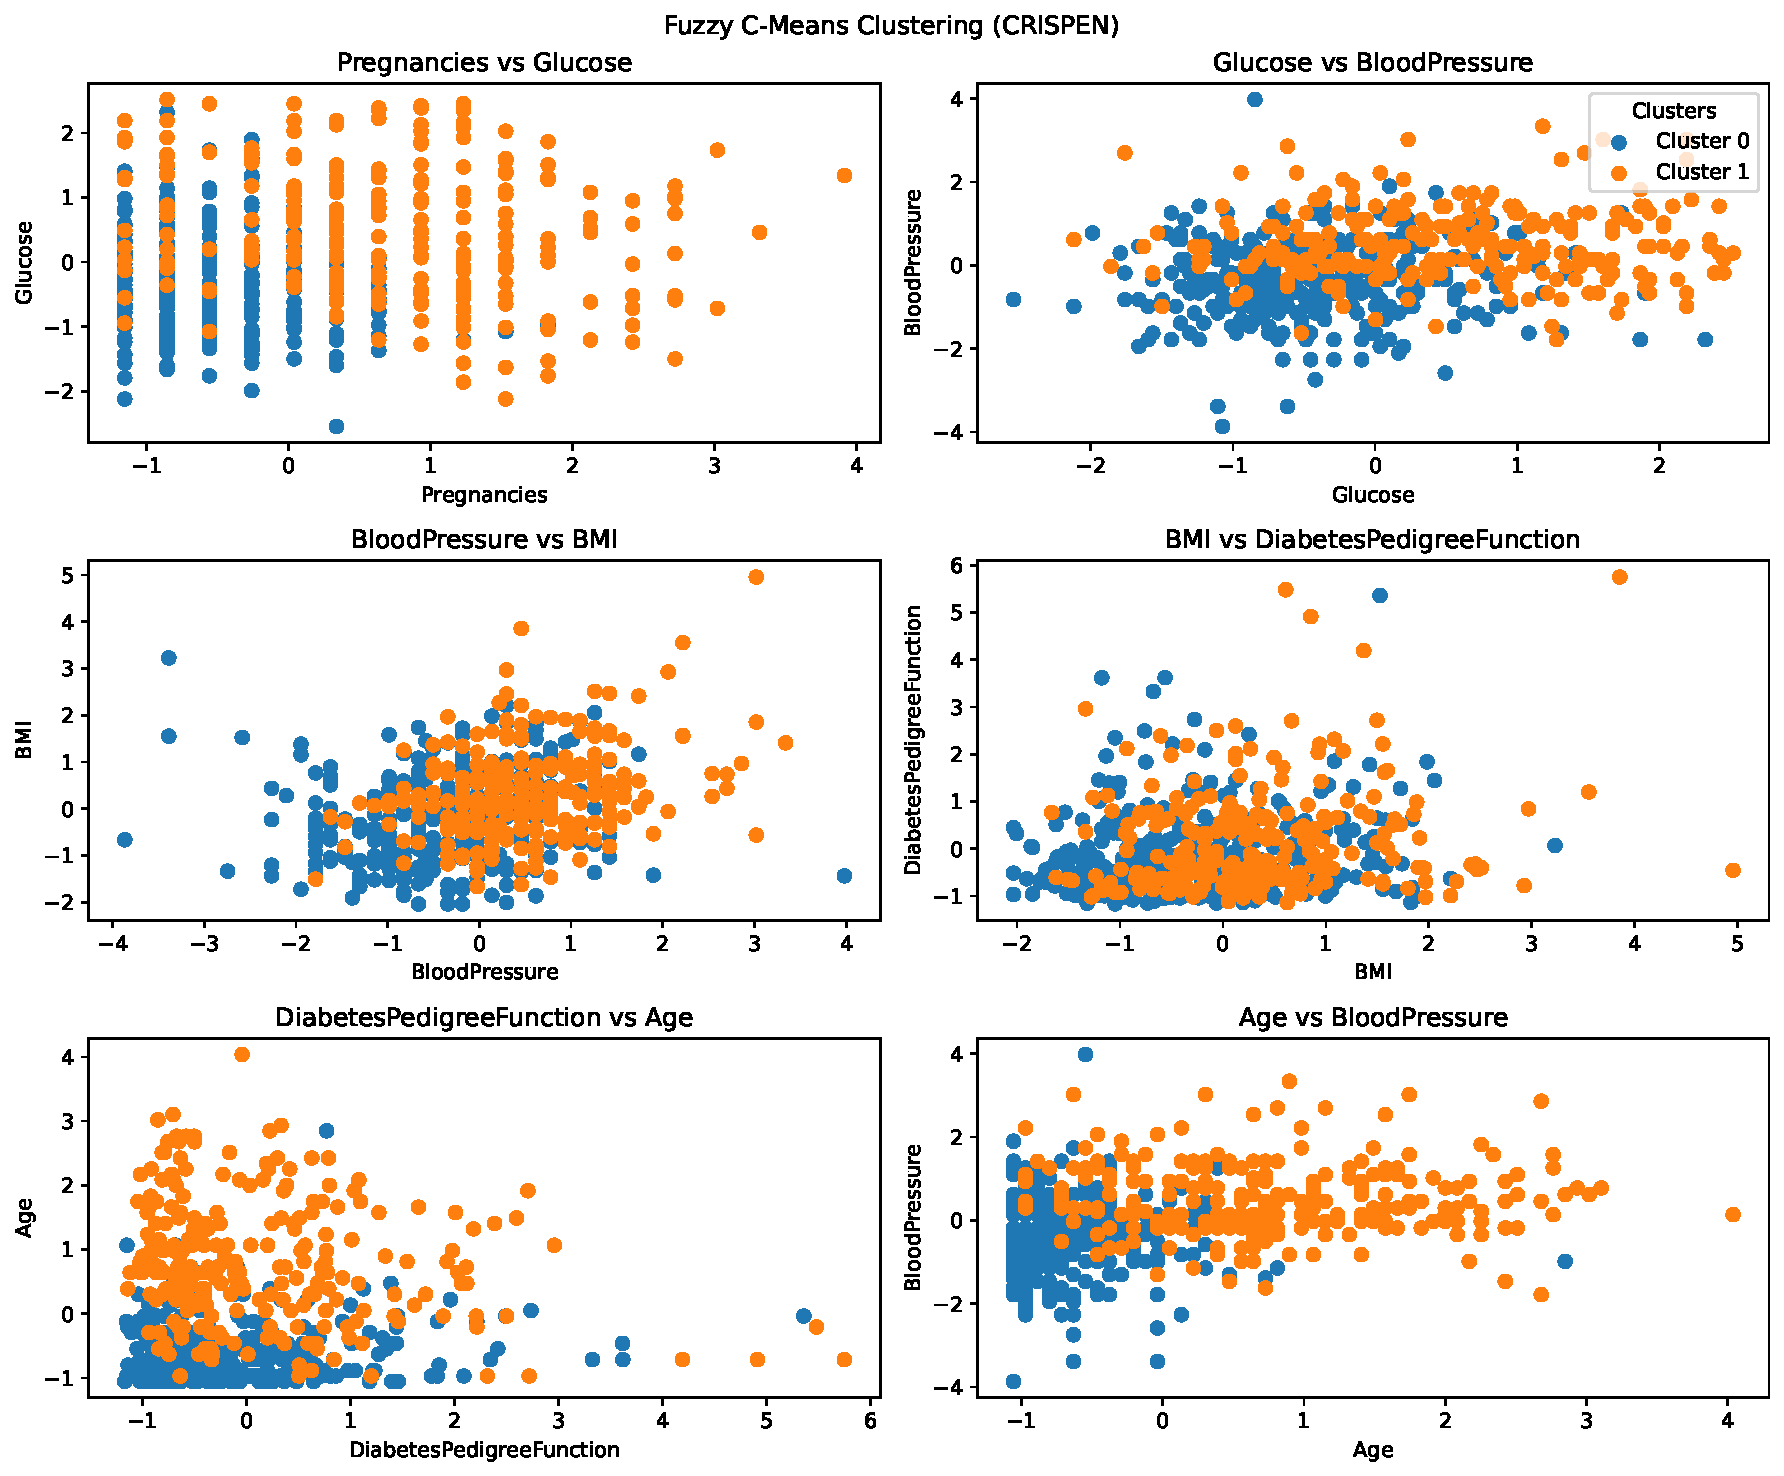
\includegraphics[width=1\textwidth]{Plots/Fuzzy C-Means Clustering (CRISPEN) CLF.pdf}
    \caption{Fuzzy C-Means Clustering (CRISPEN)}
    \label{fig:my_label}
\end{figure}